\documentclass[compress]{beamer}
\usepackage{multicol}
%\usetheme{Antibes}
\useoutertheme[footline=authortitle, subsection=true]{miniframes}
\useinnertheme{circles}
\usecolortheme{spruce}
\usefonttheme{structurebold}
\usepackage[utf8]{inputenc}
%\usepackage{titlesec}
\usepackage{amsmath}
\usepackage{mathspec}
%\setcounter{section}{2}
\setcounter{tocdepth}{1}
\usepackage{graphicx}
\usepackage{soul}
\usepackage{hyperref}
%\usepackage[justification=centering]{caption}
\graphicspath{ {./images/} }
%\usepackage[backend=biber, citestyle=numeric-comp, bibstyle=numeric, sorting=none]{biblatex}
%\addbibresource{ref.bib}
%\usepackage{fontspec}   %加這個就可以設定字體
\usepackage{xeCJK}       %讓中英文字體分開設置
\setCJKmainfont{Noto Sans CJK TC} %設定中文為系統上的字型
%\newCJKfontfamily[chinesexSerif]\CJKserif{Noto Serif CJK TC}
\setmainfont{Sabon}
\setsansfont{IBM Plex Sans}
\setmathfont(Digits,Latin){Goldman Sans}
\setmonofont{Roboto Mono}
\XeTeXlinebreaklocale "zh"             %這兩行一定要加,中文才能自動換行
\XeTeXlinebreakskip = 0pt plus 1pt     %這兩行一定要加,中文才能自動換行
\renewcommand{\baselinestretch}{1.2}

\title{Cheng Po Sheng: A self introduction}
\author{鄭泊聲}
\institute{}
\date{\today}

\AtBeginSection[]
{
    
  \begin{frame}[allowframebreaks]
    
    \tableofcontents[currentsection]
    
  \end{frame}
}

% \AtBeginSubsection[]{
%     \begin{frame}[allowframebreaks]
%         \tableofcontents[currentsubsection]
%     \end{frame}
% }

\begin{document}

\begin{frame}
    \titlepage
\end{frame}

\begin{frame}[allowframebreaks]{Outline}
    \tableofcontents
\end{frame}

\begin{frame}
    \frametitle{Ben Cheng 鄭泊聲}
    \begin{columns}
        \begin{column}{0.5\linewidth}
            \begin{itemize}
                \item Diversified interests and experiences.
                \item Strong technical skills.
                \item A good communicator.
            \end{itemize}
        \end{column}
        \begin{column}{0.5\linewidth}
            \includegraphics[width = \linewidth]{YC109980 修.jpg}
        \end{column}
    \end{columns}
\end{frame}

\section{Education}
\begin{frame}
    \frametitle{Education}
    National Taiwan University. Pursuing BSc/BA of
    \begin{itemize}
        \item Bio-Mechatronics Engineering
        \item Economics
    \end{itemize}
    in a double major program.

    Expected to graduate in JUN. 2023.
\end{frame}

\begin{frame}
    \frametitle{EE related course}
    \begin{itemize}
        \item Electrical, Eletronics Engineering
        \item Engineering Mathematics
              \begin{itemize}
                  \item ODE, linear algebra, fourier transform, PDE
              \end{itemize}
        \item Pratical Data Structures and Algorithms
              \begin{itemize}
                  \item in Java
              \end{itemize}
        \item Mechatronics I-IV
              \begin{itemize}
                  \item embedded microprocessor, signal conditioning, digital circuits, system integration
              \end{itemize}
        \item BioMEMS Fabrication
        \item Intelligent Control
              \begin{itemize}
                  \item fuzzy control, genetic algorithm, neural network
              \end{itemize}
    \end{itemize}
\end{frame}

\begin{frame}
    \frametitle{ME related course}
    \begin{multicols}{2}
        \begin{itemize}
            \item Applied Mechanics I, II
            \item Strength of Materials
            \item Mechanism
            \item Design of Machine Elements
            \item Physical Chemistry
            \item Engineering Materials
            \item Fluid Mechanics
            \item Thermal Dynamics
            \item Heat Transfer
            \item Power Machinery
            \item Actuators
            \item Automatic Control
        \end{itemize}
    \end{multicols}
\end{frame}

\section{Experiences}

\subsection{Mechanical Engineering Intern, Logitech}
\begin{frame}
    \frametitle{Mechanical Engineering Intern, Logitech}
    \begin{itemize}
        \item Feb. 2022 - Jun 2022.
        \item Bringing electrical engineering skills to mechanical team to create new technology for keyboard.
        \item Involves ProE/Creo, R, SLA/3DP prototyping.
    \end{itemize}
    \begin{figure}
        \centering
        
\includegraphics[width = 0.5\linewidth]{High_Resolution_JPEG-LogitechG_horz_RGB_cyan_LG.jpg}
    \end{figure}
\end{frame}

\subsection{College Student Researcher, CCMS, NTU}
\begin{frame}
    \frametitle{College Student Researcher, CCMS, NTU}
    \begin{itemize}
        \item Jul. 2021 - Feb. 2022.
        \item Develope a novel spectral measurement and mapping system that integrates several components with LabVIEW. \href{https://bencer3283.github.io/experiences/collegeStudentResearch/}{\underline{Details linked here.}}
        \item Also involves Flutter/Dart, UI/UX, C++, optics engineering, hyperspectral image processing.
        \item The project won an Excellance Awards (NT20,000) at 2021 CCMS Innovative Techniques Competition.
    \end{itemize}
\end{frame}

\begin{frame}
    \begin{columns}
        \begin{column}{0.4\linewidth}
            Some results from this project (links):
            \begin{itemize}
                \item \href{https://github.com/HyperSpectral-Imaging}{Github Repos}
                \item \href{https://github.com/HyperSpectral-Imaging/HSI-docs/raw/main/final.pdf}{MOST Final report}
                \item \href{https://cheng-posheng.gitbook.io/hsi-main-project-api-documentation/}{LabVIEW Source Code Documentation}
            \end{itemize}
        \end{column}
        \begin{column}{0.6\linewidth}
            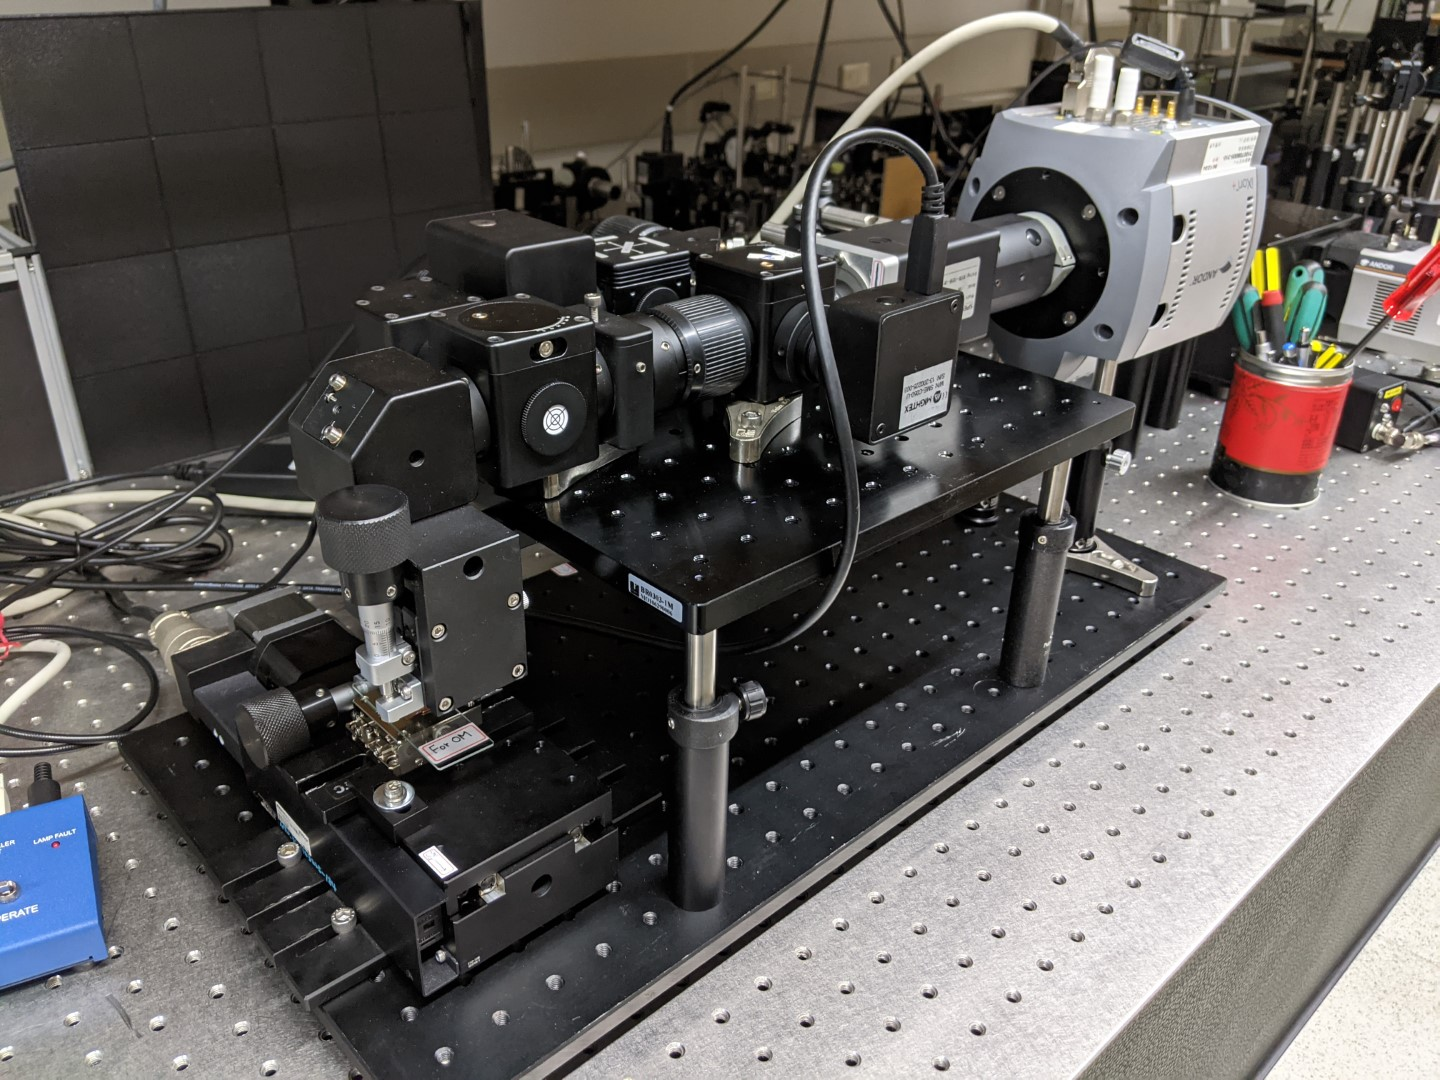
\includegraphics[width=\linewidth]{microSystemPixel3.jpg}
        \end{column}
    \end{columns}
\end{frame}

\subsection{IoT Farm Feild Pest Monitoring Device}
\begin{frame}
    \frametitle{IoT Farm Feild Pest Monitoring Device}
    \begin{columns}
        \begin{column}{0.5\linewidth}
            \begin{itemize}
                \item A self-directed project. May 2020 - present, @Bio-Electromagnetics Lab, NTU
                \item Design a IoT-connected machine to monitor the amount of bugs in farm fields with \href{https://bencer3283.github.io/experiences/Iot/}{\underline{self-designed}} controller board and mechanics.
            \end{itemize}
        \end{column}
        \begin{column}{0.5\linewidth}
            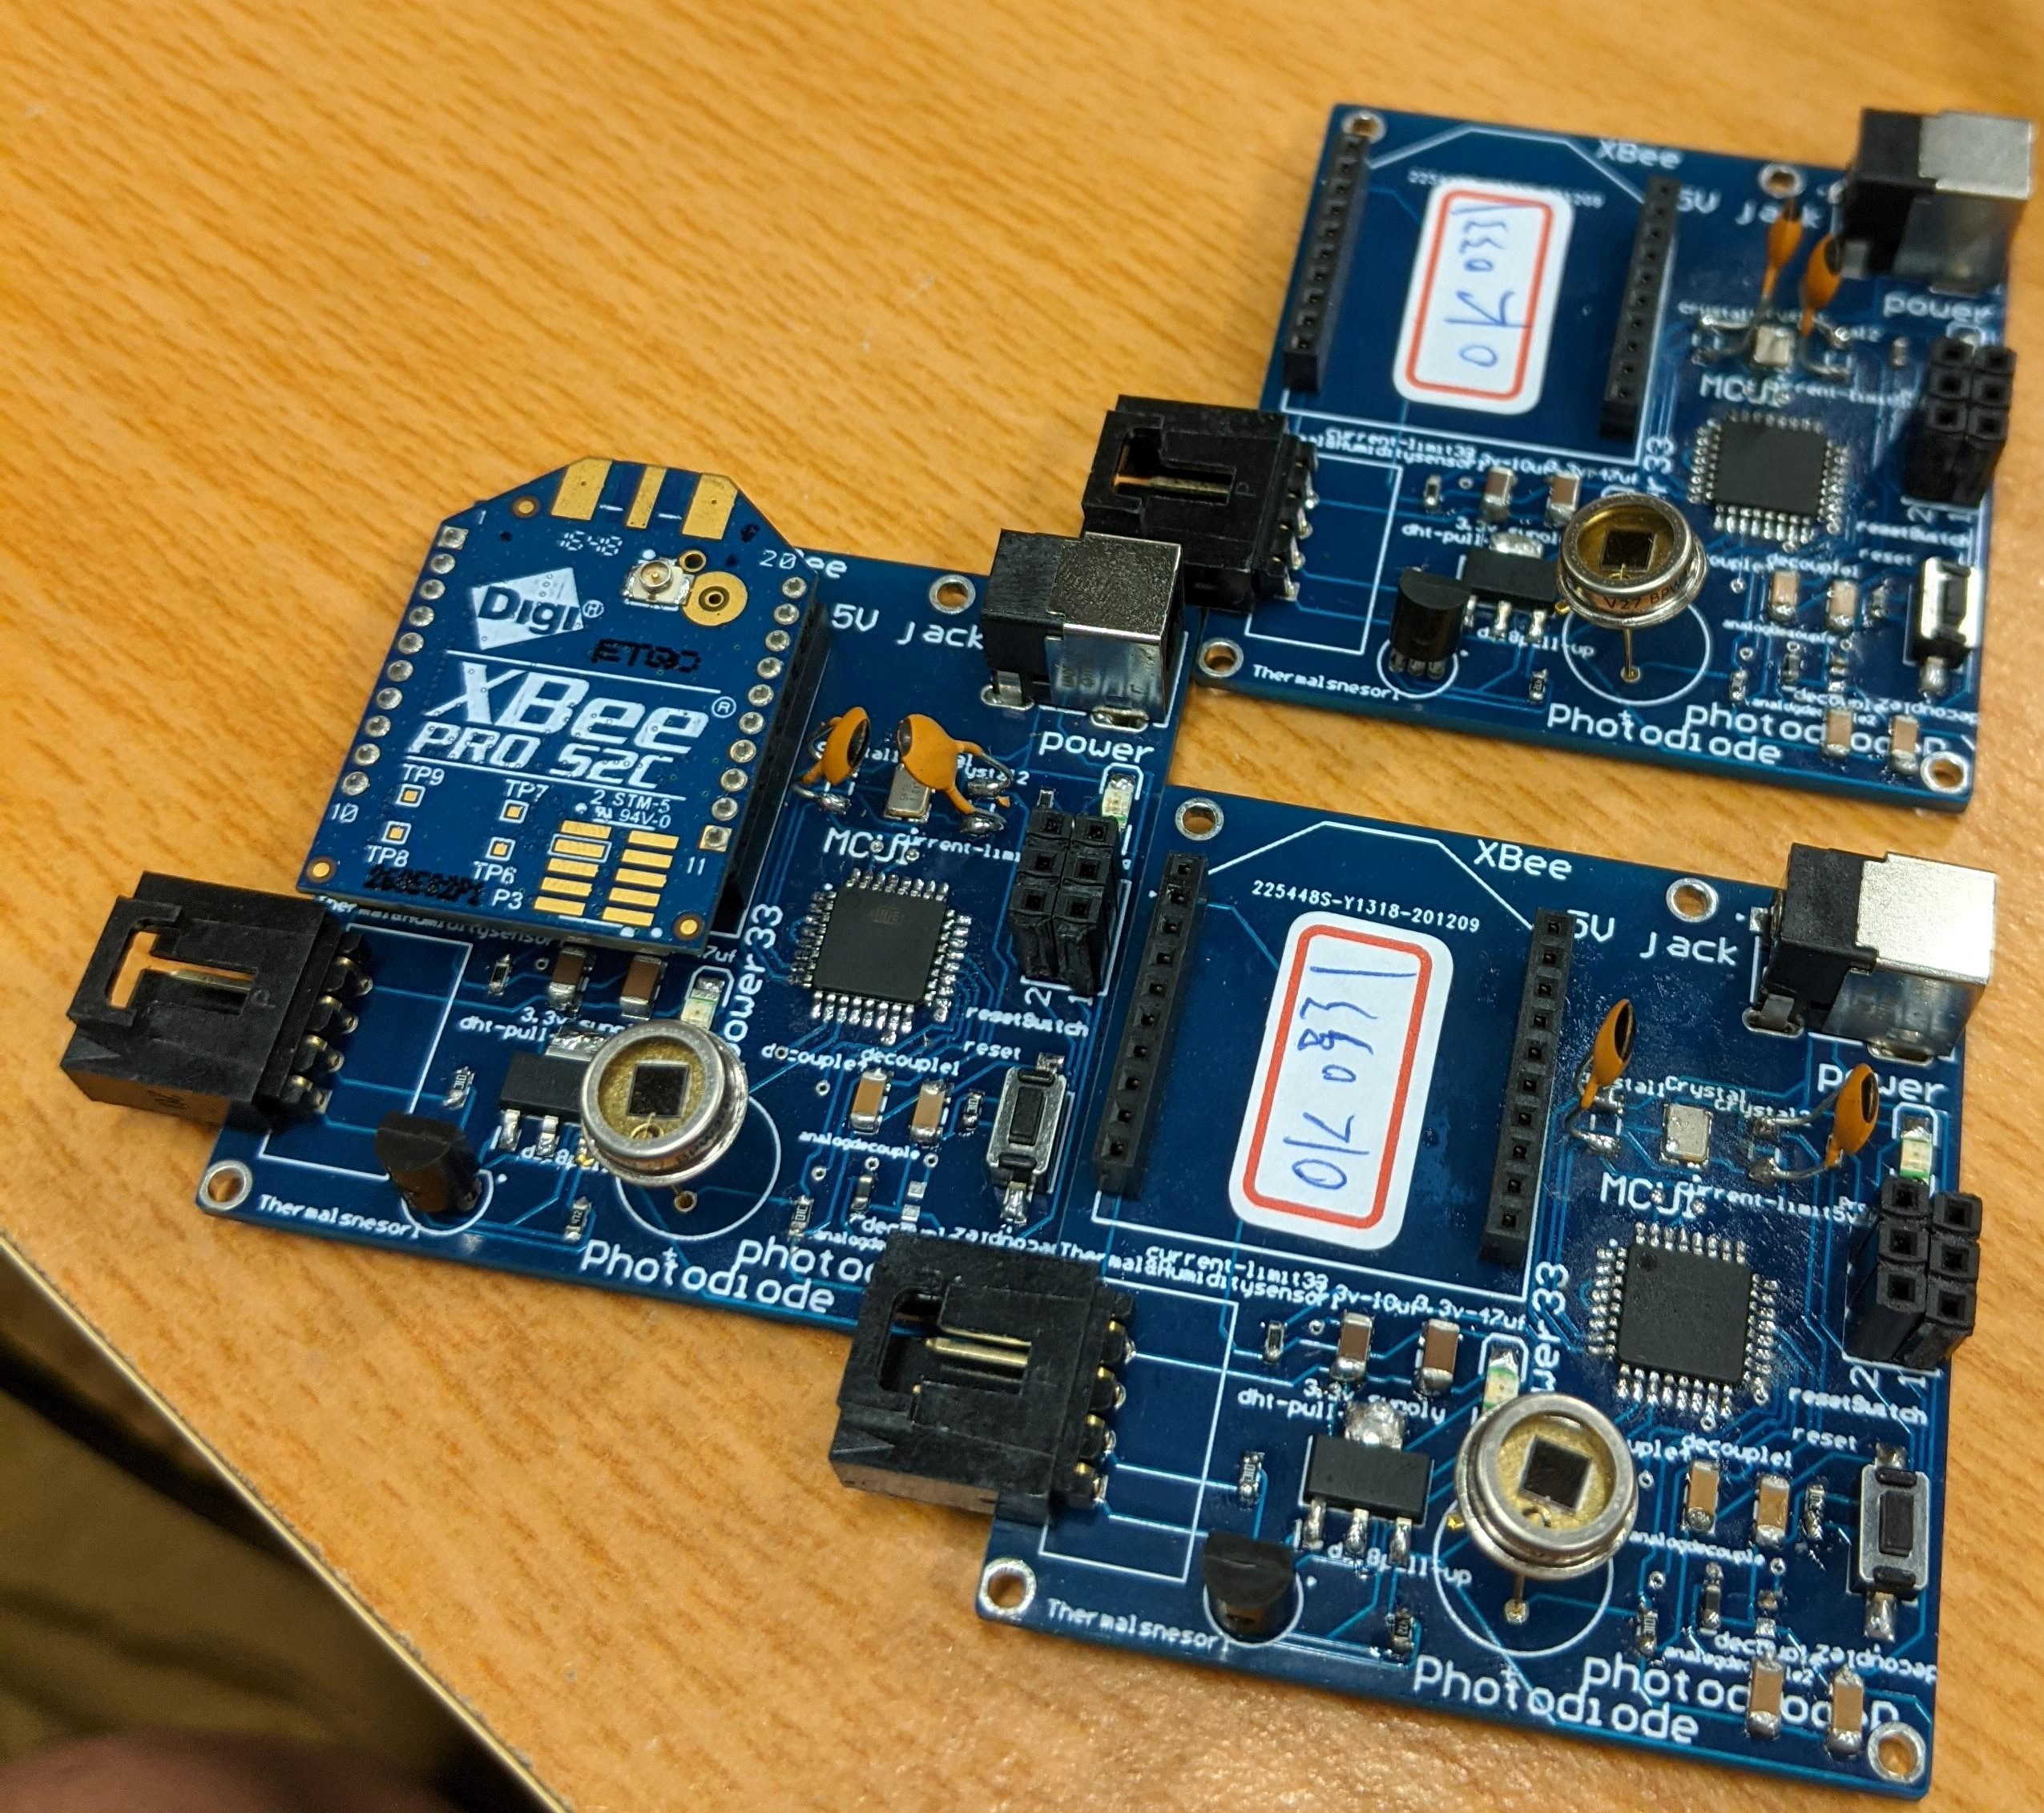
\includegraphics[width=\linewidth]{3pGto7b.jpg}
        \end{column}
    \end{columns}
\end{frame}

\begin{frame}
    \begin{columns}
        \begin{column}{0.5\linewidth}
            \begin{itemize}
                \item Involves mechatronics, IoT (XBee), PCB design (Altium), Python, SolidWorks, microprocessor, Raspberry Pi, MySQL.
            \end{itemize}
        \end{column}
        \begin{column}{0.5\linewidth}
            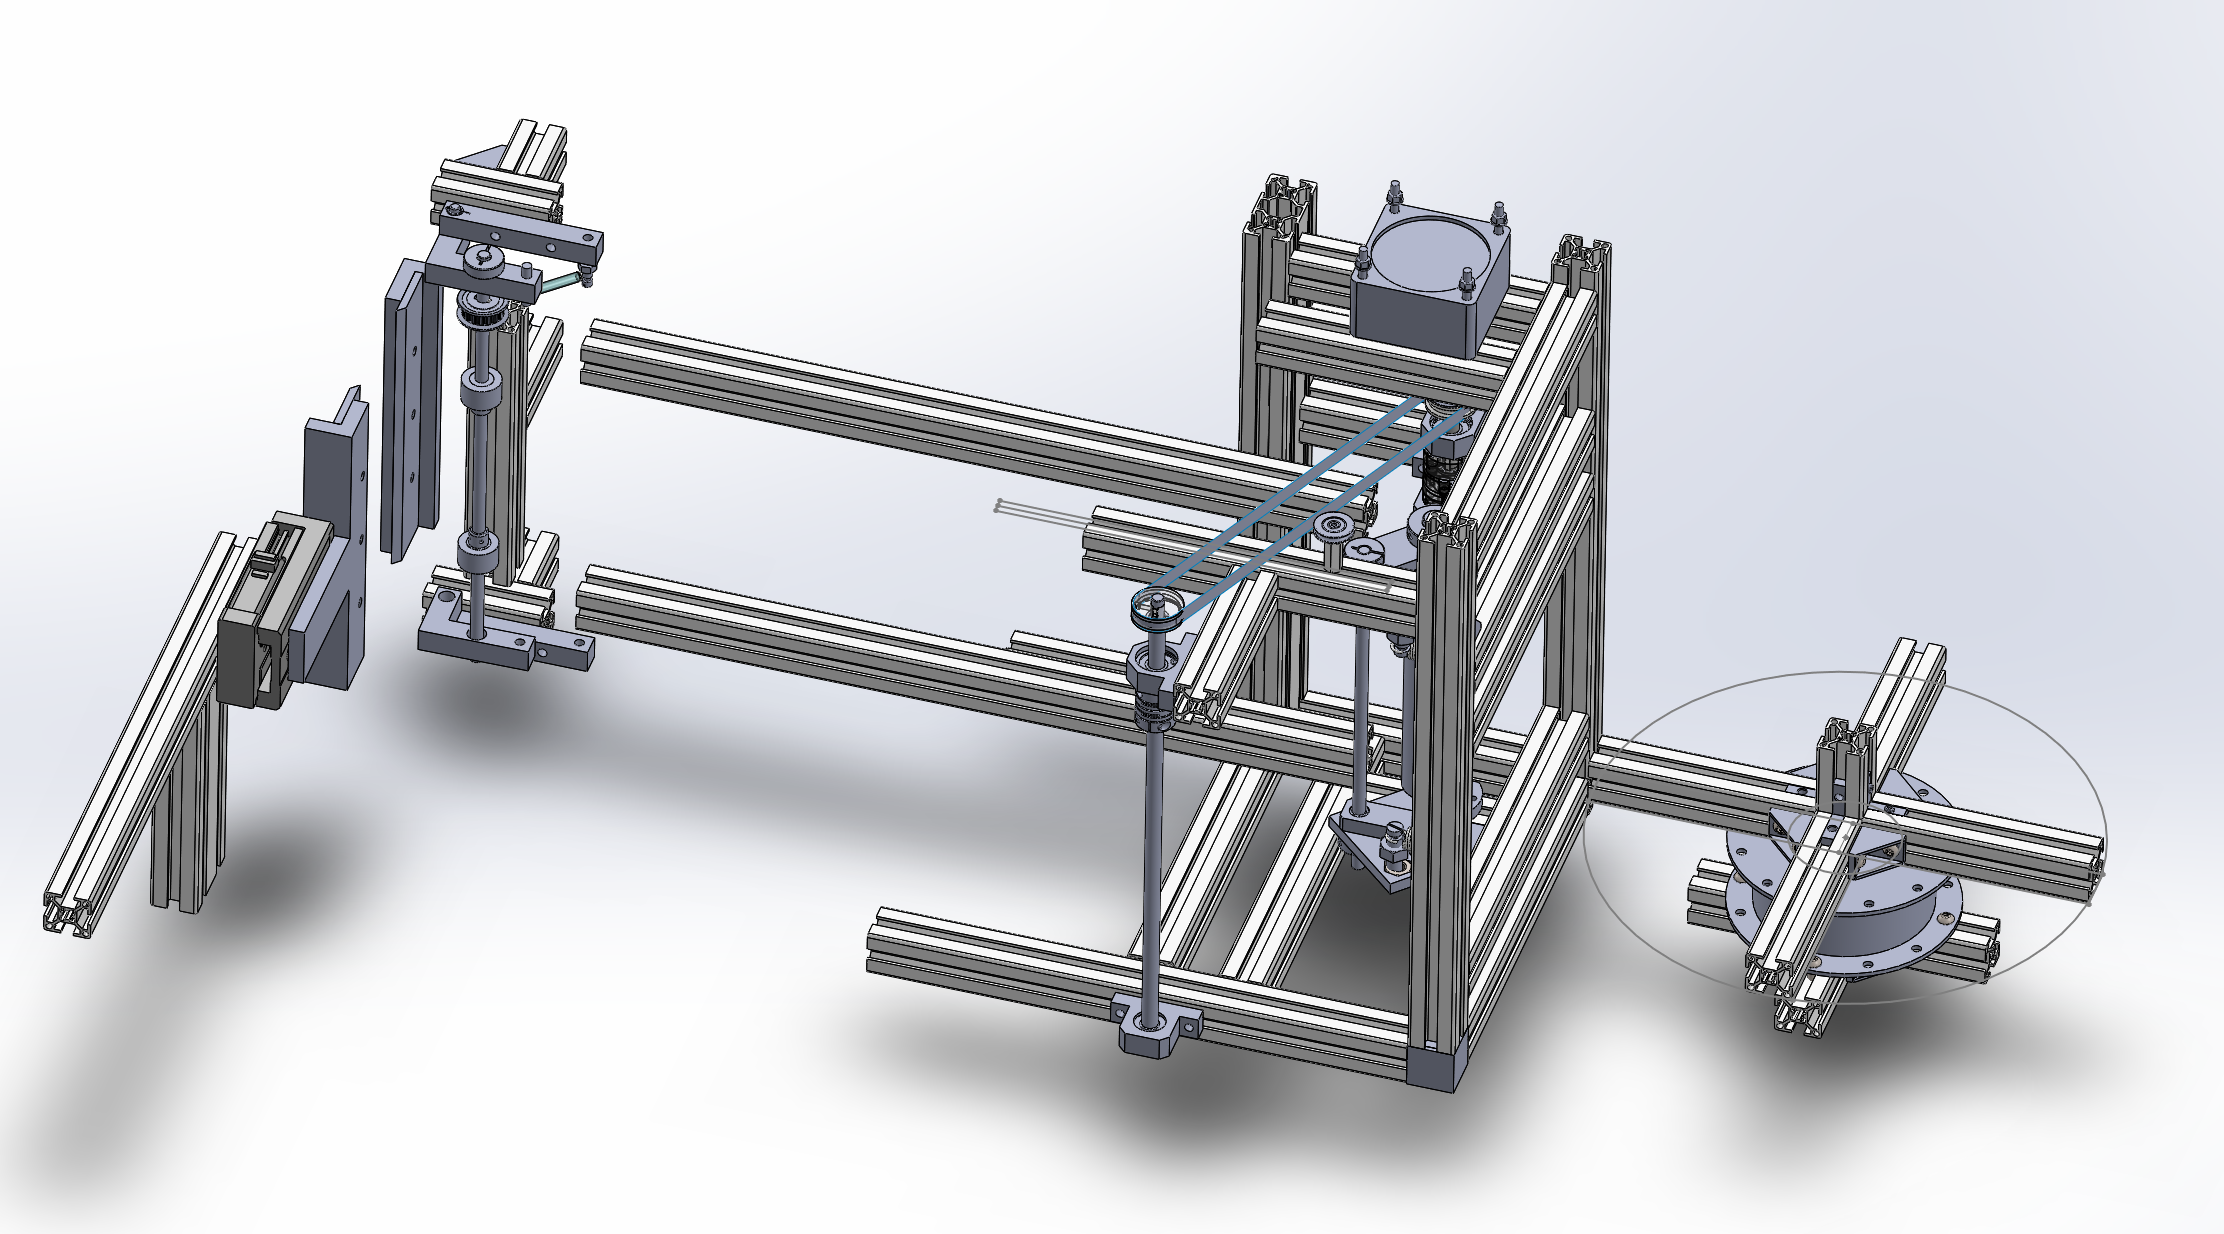
\includegraphics[width=\linewidth]{pestMachine.png}
        \end{column}
    \end{columns}
\end{frame}

\subsection{Golden medalist, 19th Mobileheroes Award}
\begin{frame}
    \frametitle{Golden medalist, 19th Mobileheroes Award}
    \begin{itemize}
        \item Category of 5G innovative application, (NT300,000) awarded by Industrial Development Bureau.
        \item Our team ARGO has developed a AR platform that utilize advanced image-based spacial recognition algorithm that enables complex AR experiences on personal mobile devices.
        \item My main contribution are UI/UX evaluation and design of the AR world for demo.
    \end{itemize}
\end{frame}

\subsection{Championship Thesis on Industrial Impact of COVID}
\begin{frame}
    \frametitle{Championship, 2021 National Thesis Competition for College Students}
    \begin{itemize}
        \item "Covid-19's Impact on Online Video Streaming Platform from The Perspective of Consumer Preference"
        \item In this work we found that most consumers didn't think the pandemic makes than more prone to subscription video services. By our statistics analysis, we found that only "family plan", which reduces price substentially, can make consumers prefer subscription OTT platform.
        \item Involves Matlab for statistics (Chi-square test for independence,
              Logistic regression).
    \end{itemize}
\end{frame}




\section{Personalities}
\subsection{Curiosity with breadth and depth}
\subsection{A self-directed learner}
\subsection{A good listener}

\end{document}